\documentclass[aspectratio=169]{beamer}
\usepackage[utf8]{inputenc}
\usepackage[T1]{fontenc}
\usepackage{lmodern}
\usepackage{xcolor}
\usepackage[portuguese]{babel}
\usepackage{amsmath}

\definecolor{BgCream}{HTML}{FAF8F5}
\definecolor{TextEspresso}{HTML}{4A4238}
\definecolor{NudeTaupe}{HTML}{BFAFA6}
\definecolor{SoftBlush}{HTML}{D9C5B2}

\setbeamertemplate{navigation symbols}{}
\setbeamercolor{background canvas}{bg=BgCream}
\setbeamercolor{normal text}{fg=TextEspresso}
\setbeamercolor{structure}{fg=TextEspresso}

\setbeamertemplate{itemize item}{\color{NudeTaupe}\textendash}
\setbeamertemplate{itemize subitem}{\color{NudeTaupe}\(\circ\)}

\setbeamerfont{title}{size=\huge, series=\bfseries}
\setbeamerfont{frametitle}{size=\Large, series=\bfseries}

\setbeamertemplate{title page}{
  \vspace*{1.5cm}
  \begin{center}
    \usebeamerfont{title}\textcolor{TextEspresso}{\inserttitle}\par
    \vspace{0.35cm}
    {\large\textcolor{NudeTaupe}{\insertsubtitle}}\par
    \vspace{0.6cm}
    {\color{NudeTaupe}\rule{2.5cm}{0.5pt}}\par
    \vspace{0.8cm}
    \usebeamerfont{author}\textcolor{TextEspresso}{\insertauthor}\par
    \vspace{0.3cm}
    \usebeamerfont{institute}\small\textcolor{NudeTaupe}{\insertinstitute \quad|\quad \insertdate}
  \end{center}
}

\setbeamertemplate{frametitle}{
  \vspace*{0.8cm}
  \usebeamerfont{frametitle}\insertframetitle\par
  \vspace*{-0.1cm}
  {\color{NudeTaupe}\rule{1.5cm}{0.5pt}}
  \vspace*{0.2cm}
}

\newenvironment{ideiachave}{
  \vspace{0.5cm}
  \begin{center}
  \color{TextEspresso}
  \itshape\Large
}{
  \end{center}
  \vspace{0.5cm}
}

\newcommand{\seccao}[2]{%
  \begin{frame}[plain]
    \vspace*{2.2cm}
    \begin{center}
      {\color{NudeTaupe}\rule{3cm}{0.5pt}}\par
      \vspace{0.6cm}
      {\Huge\bfseries\textcolor{TextEspresso}{#1}}\par
      \vspace{0.5cm}
      {\large\textcolor{NudeTaupe}{#2}}\par
      \vspace{0.6cm}
      {\color{NudeTaupe}\rule{3cm}{0.5pt}}
    \end{center}
  \end{frame}
}


\newcommand{\casodiscussao}[3]{%
  \begin{frame}
  \frametitle{#1}
  \begin{itemize}
      \setlength\itemsep{0.35cm}
      #2
  \end{itemize}
  \vspace{0.25cm}
  {\small\color{NudeTaupe}\textbf{15 minutos} para pensar em grupo, seguidos de discussão. #3}
  \end{frame}
}

\usepackage{csquotes}

\title{Fundamentos de Infraestruturas de Computação na Nuvem}
\subtitle{Infraestruturas de Computação na Nuvem, Aula 01}
\author{Catarina Silva}
\institute{ESTGA, Universidade de Aveiro}
\date{2026}

\begin{document}

\begin{frame}[plain]
  \titlepage
\end{frame}


\seccao{Parte 1}{O objeto de estudo}

\begin{frame}
\frametitle{O que distingue uma infraestrutura}
\begin{itemize}
    \setlength\itemsep{0.35cm}
    \item Uma infraestrutura caracteriza-se por ser \textbf{partilhada}, \textbf{persistente} e \textbf{transparente em funcionamento normal}.
    \item Partilhada: serve múltiplos consumidores que não coordenam entre si.
    \item Persistente: a sua escala de tempo é superior à das aplicações que suporta.
    \item Transparente: quando funciona bem, ninguém repara nela. Torna-se visível apenas na falha -- o que tem consequências para a forma como é financiada e valorizada.
\end{itemize}
\end{frame}

\begin{frame}
\frametitle{O problema}
\begin{itemize}
    \setlength\itemsep{0.4cm}
    \item Existe um conjunto \emph{finito} de recursos físicos e um conjunto \emph{variável} de procuras concorrentes sobre eles.
    \item Toda a disciplina decorre da tensão entre estes dois factos.
    \item As perguntas que atravessam o semestre são sempre variações da mesma: \emph{como se reparte um recurso escasso entre consumidores que não confiam uns nos outros, de forma eficiente, previsível e resistente a falhas?}
\end{itemize}
\begin{ideiachave}
Partilhar sem interferir.
\end{ideiachave}
\end{frame}

\begin{frame}
\frametitle{Tipos de recurso}
\begin{itemize}
    \setlength\itemsep{0.3cm}
    \item \textbf{Recurso}: entidade finita cujo consumo por um utilizador reduz a disponibilidade para os restantes.
    \item Distinguem-se pela forma como se esgotam e se recuperam:
    \begin{itemize}
      \item \textbf{Renováveis por tempo} -- processador, largura de banda. Não usar num instante é desperdício irrecuperável.
      \item \textbf{Ocupacionais} -- memória, espaço em disco. Mantêm-se ocupados até serem libertados.
    \end{itemize}
    \item Esta distinção determina que mecanismo de partilha é aplicável a cada recurso.
\end{itemize}
\end{frame}

\begin{frame}
\frametitle{Dois mecanismos de partilha}
\begin{itemize}
    \setlength\itemsep{0.35cm}
    \item \textbf{Multiplexagem temporal}: o recurso é atribuído integralmente a um consumidor de cada vez, alternando no tempo. Aplica-se a recursos renováveis por tempo.
    \item \textbf{Multiplexagem espacial}: o recurso é dividido em porções atribuídas simultaneamente. Aplica-se a recursos ocupacionais.
    \item A comutação temporal tem um custo de \emph{troca de contexto}; a divisão espacial tem um custo de \emph{fragmentação}.
    \item Praticamente todos os mecanismos que estudaremos são combinações destes dois, aplicadas a níveis diferentes de abstração.
\end{itemize}
\end{frame}

\begin{frame}
\frametitle{Multiplexagem temporal e espacial}
\vfill
\begin{center}
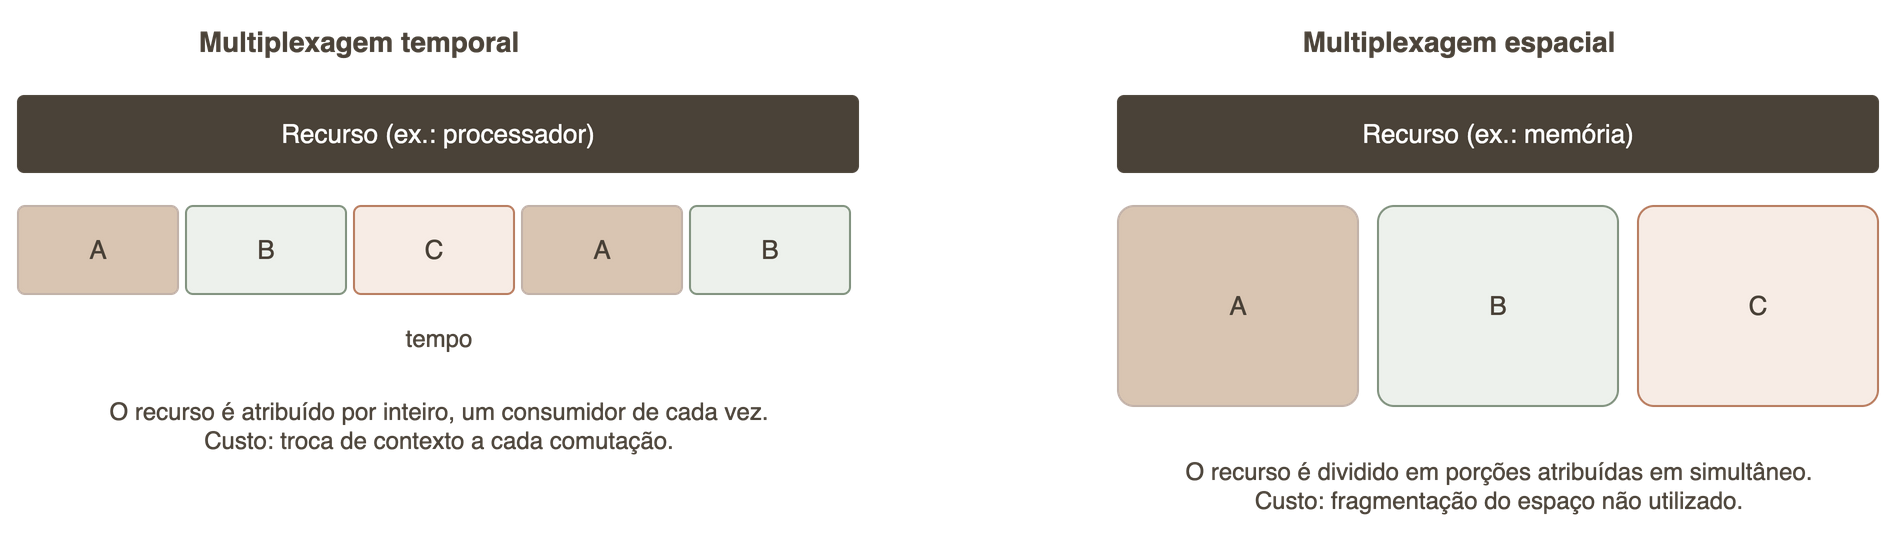
\includegraphics[width=0.97\textwidth,height=0.70\textheight,keepaspectratio]{../Diagramas/a01-multiplexagem.png}
\end{center}
\vfill
\end{frame}

\begin{frame}
\frametitle{Virtualizar não é só criar VMs}
\begin{itemize}
    \setlength\itemsep{0.35cm}
    \item \textbf{Virtualizar} é apresentar a um consumidor uma interface que se comporta como um recurso dedicado, sendo na realidade uma parte de um recurso partilhado.
    \item O conceito não se restringe a máquinas virtuais: memória virtual, sistemas de ficheiros e endereçamento de rede são todos instâncias do mesmo princípio.
    \item Requer três capacidades: \emph{traduzir} referências virtuais em físicas, \emph{arbitrar} o acesso concorrente e \emph{isolar} os consumidores entre si.
    \item Quando qualquer uma das três falha, a abstração deixa de se sustentar -- e o comportamento torna-se difícil de explicar a partir da interface.
\end{itemize}
\end{frame}

\begin{frame}
\frametitle{A virtualização não é uma técnica recente}
\begin{itemize}
    \setlength\itemsep{0.35cm}
    \item Os mainframes IBM System/360, na década de 1960, já particionavam um único computador entre múltiplos sistemas operativos monoutilizador -- o antecedente direto da máquina virtual atual.
    \item O interesse esmoreceu nos anos 1980 e 1990, quando os sistemas operativos multiutilizador tornaram redundante grande parte dessa necessidade.
    \item Foi retomada a partir de 1998, com a VMware, e consolidada entre 2005 e 2008 com suporte de hardware dedicado (Intel VT-x, AMD-V) e hypervisors como Xen e KVM.
    \item É esta maturação de várias décadas -- não uma inovação recente -- que sustenta o modelo de \emph{cloud} elástica discutido na Parte 4.
\end{itemize}
\end{frame}

\begin{frame}
\frametitle{A definição formal de Popek e Goldberg}
\begin{itemize}
    \setlength\itemsep{0.28cm}
    \item Referência clássica: Gerald J. Popek e Robert P. Goldberg, \emph{Formal Requirements for Virtualizable Third Generation Architectures}, Communications of the ACM, 1974.
    \item Os autores formalizam a exigência de isolamento enunciada atrás: um \emph{Virtual Machine Monitor} pode ser construído sempre que o conjunto de instruções sensíveis de uma arquitetura for subconjunto do conjunto de instruções privilegiadas.
    \item Quando essa condição falha -- como sucedia em arquiteturas x86 anteriores a 2005 --, algumas instruções sensíveis não geram exceção, e o isolamento tem de ser assegurado por outros meios.
    \item O resultado é uma condição verificável sobre uma arquitetura de processador, e não uma propriedade de um produto concreto.
\end{itemize}
\end{frame}

\begin{frame}
\frametitle{Hypervisor: duas arquiteturas}
\begin{itemize}
    \setlength\itemsep{0.35cm}
    \item \textbf{Hypervisor}: o componente que implementa a multiplexagem de hardware entre máquinas virtuais.
    \item \textbf{Tipo 1 (nativo)} -- executa diretamente sobre o hardware, sem sistema operativo hospedeiro. Exemplos: Xen, KVM, VMware ESXi.
    \item \textbf{Tipo 2 (alojado)} -- executa como aplicação sobre um sistema operativo hospedeiro, que continua a mediar o acesso ao hardware. Exemplo: VirtualBox.
    \item A diferença é, também ela, uma questão de indirecção: o tipo 2 introduz uma camada adicional -- o sistema operativo hospedeiro -- entre o hypervisor e o hardware.
\end{itemize}
\end{frame}

\begin{frame}
\frametitle{Duas arquiteturas de hypervisor}
\vfill
\begin{center}
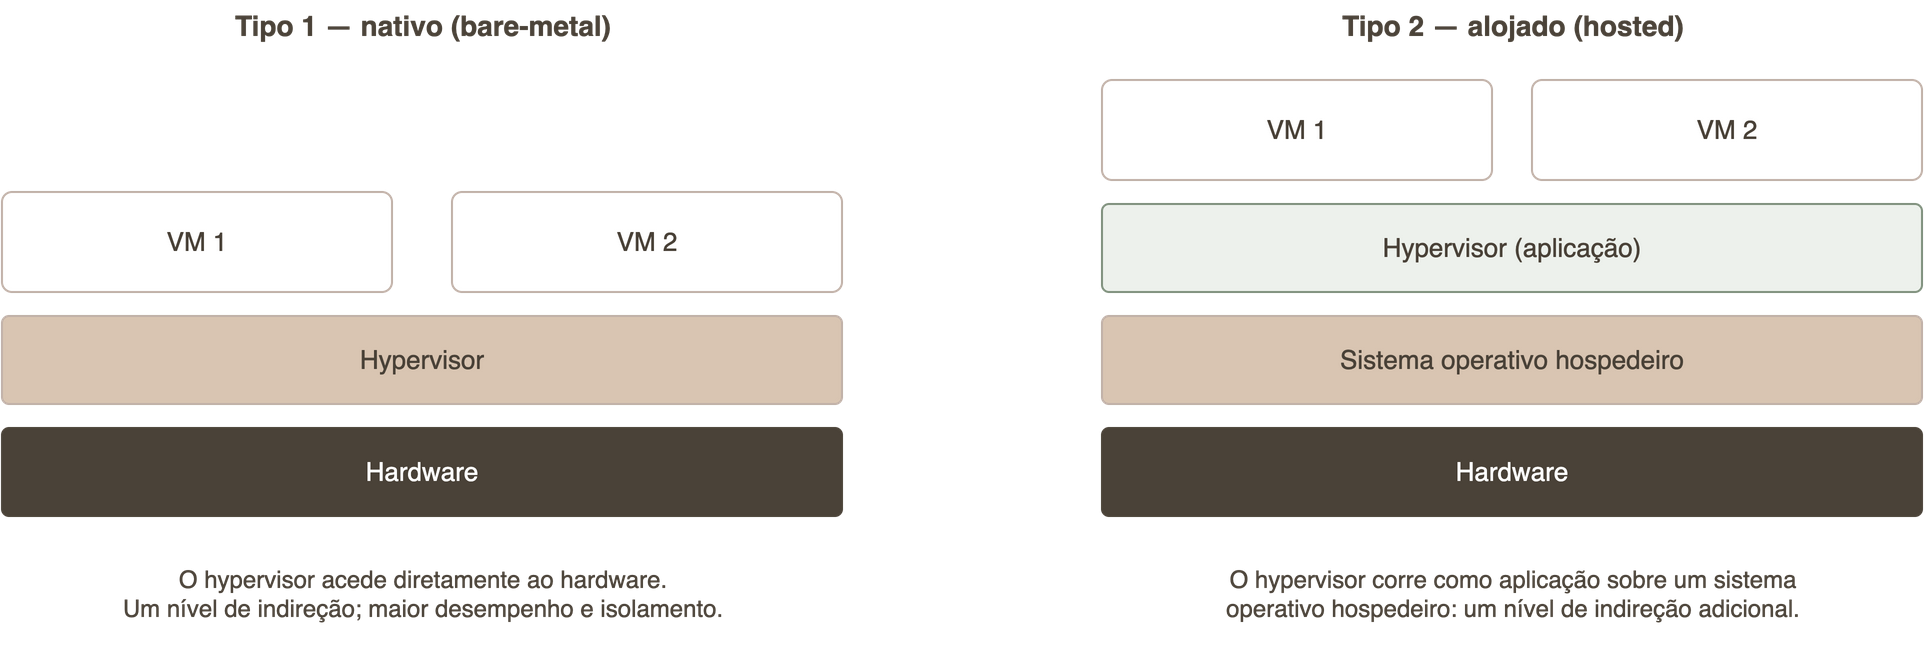
\includegraphics[width=0.97\textwidth,height=0.70\textheight,keepaspectratio]{../Diagramas/a01-hypervisor-tipos.png}
\end{center}
\vfill
\end{frame}

\begin{frame}
\frametitle{Acrescentar um nível de indirecção}
\begin{itemize}
    \setlength\itemsep{0.35cm}
    \item Introduzir um nível de indirecção significa deixar de referir um recurso diretamente e passar a referi-lo através de um intermediário que faz a tradução.
    \item É o que permite substituir, mover ou replicar o recurso sem alterar quem o refere.
    \item Praticamente todas as propriedades que valorizamos -- portabilidade, elasticidade, tolerância a falhas -- decorrem da existência dessa camada intermédia.
    \item Formulação clássica, atribuída a David Wheeler: qualquer problema em informática pode ser resolvido acrescentando um nível de indirecção.
\end{itemize}
\end{frame}

\begin{frame}
\frametitle{O que a indirecção custa}
\begin{itemize}
    \setlength\itemsep{0.35cm}
    \item A mesma formulação costuma ser completada com uma ressalva: o problema que a indirecção não resolve é o de haver indirecção a mais.
    \item Cada camada acrescenta latência, consome recursos e introduz um novo modo de falha.
    \item Acrescenta também \textbf{opacidade}: o diagnóstico passa a exigir atravessar todas as camadas.
    \item Decisão de engenharia recorrente nesta UC: \emph{que indirecção compensa introduzir, e a que custo}.
    \item Não existe resposta universal -- depende dos requisitos de cada sistema.
\end{itemize}
\end{frame}

% ============================================================
\seccao{Parte 2}{Princípios de arquitetura}

\begin{frame}
\frametitle{Onde as abstrações falham}
\begin{itemize}
    \setlength\itemsep{0.35cm}
    \item Uma abstração é um contrato: expõe um conjunto de operações e oculta a forma como são realizadas.
    \item O seu valor está no que oculta; a sua fragilidade está exatamente no mesmo sítio.
    \item \textbf{Abstrações com fugas}: propriedades da implementação que se tornam observáveis através da interface -- tipicamente o desempenho.
    \item Um disco virtual comporta-se como um disco até o armazenamento subjacente saturar. A interface não mudou; o comportamento sim.
    \item Consequência prática: o administrador de infraestrutura tem de compreender \emph{pelo menos uma camada abaixo} daquela em que opera.
\end{itemize}
\end{frame}

\begin{frame}
\frametitle{Mecanismo e política}
\begin{itemize}
    \setlength\itemsep{0.35cm}
    \item \textbf{Mecanismo}: o que o sistema é \emph{capaz} de fazer. \textbf{Política}: o que o sistema \emph{deve} fazer em cada circunstância.
    \item Separá-los permite alterar a política sem reimplementar o sistema.
    \item Exemplo estrutural: um orquestrador fornece o mecanismo de colocar cargas de trabalho em nós; a política de colocação é declarada à parte, pelo operador.
    \item É este princípio que torna uma plataforma \emph{configurável} em vez de meramente \emph{programável}.
    \item Reaparecerá em praticamente todos os blocos do programa.
\end{itemize}
\end{frame}

\begin{frame}
\frametitle{O argumento end-to-end}
\begin{itemize}
    \setlength\itemsep{0.35cm}
    \item Já vem do contexto do desenho de sistemas distribuídos.
    \item Uma função só pode ser garantida de forma completa e correta com conhecimento que reside nos \emph{extremos} da comunicação.
    \item Implementá-la em camadas intermédias é, no limite, redundante -- ainda que possa justificar-se por razões de desempenho.
    \item Consequência para infraestrutura: a camada de infraestrutura não deve tentar garantir propriedades que só a aplicação pode assegurar.
    \item Delimita o que é razoável exigir de uma plataforma, e o que tem de permanecer responsabilidade de quem a usa.
\end{itemize}
\end{frame}

\begin{frame}
\frametitle{Declarativo vs imperativo}
\begin{itemize}
    \setlength\itemsep{0.35cm}
    \item \textbf{Imperativa}: descreve-se a \emph{sequência de ações} a executar. O resultado depende do estado inicial.
    \item \textbf{Declarativa}: descreve-se o \emph{estado final pretendido}. Cabe ao sistema determinar as ações necessárias.
    \item A forma declarativa é composicional e verificável: pode comparar-se a especificação com a realidade observada.
    \item A forma imperativa não o permite -- um conjunto de comandos não se compara com um estado.
    \item Esta distinção é o fundamento conceptual da automatização moderna de infraestrutura.
\end{itemize}
\end{frame}

\begin{frame}
\frametitle{Idempotência e convergência}
\begin{itemize}
    \setlength\itemsep{0.35cm}
    \item Uma operação é \textbf{idempotente} se o efeito de a aplicar $n$ vezes é indistinguível do de a aplicar uma vez.
    \item Formalmente: $f(f(x)) = f(x)$ para todo o $x$ do domínio.
    \item A idempotência é o que permite \emph{repetir com segurança} -- e repetir com segurança é o que permite recuperar de falhas parciais sem raciocinar sobre o ponto exato em que a execução foi interrompida.
    \item \textbf{Convergência}: propriedade de um sistema que, aplicando repetidamente a mesma especificação, tende para o estado declarado.
    \item Sem idempotência, a repetição é perigosa; sem repetição, não há convergência.
\end{itemize}
\end{frame}

\begin{frame}
\frametitle{Idempotência na prática}
\begin{itemize}
    \setlength\itemsep{0.3cm}
    \item Suponha um procedimento que acrescenta um servidor a um ficheiro de configuração de um balanceador de carga.
    \item \textbf{Versão não idempotente}: «acrescentar a linha \texttt{server 10.0.0.7} ao ficheiro». Correr duas vezes deixa a linha duplicada; o balanceador pode recusar arrancar.
    \item \textbf{Versão idempotente}: «garantir que o ficheiro contém exatamente estes três servidores». Correr as vezes que forem necessárias produz sempre o mesmo ficheiro.
    \item A diferença aparece quando a execução falha a meio: com a primeira versão é preciso descobrir onde parou; com a segunda, basta repetir.
    \item É por isso que as ferramentas de automatização que veremos em C3 descrevem \emph{estado}, e não sequências de comandos.
\end{itemize}
\end{frame}

\begin{frame}
\frametitle{Controlo em malha fechada}
\begin{itemize}
    \setlength\itemsep{0.35cm}
    \item Vários sistemas que estudaremos são, estruturalmente, \textbf{controladores em malha fechada}.
    \item Elementos: um \emph{valor de referência} (estado desejado), uma \emph{medição} (estado observado), um \emph{erro} (a diferença) e uma \emph{ação} que tende a reduzi-lo.
    \item A execução é contínua, não episódica: o sistema não «faz» e termina -- observa e corrige indefinidamente.
    \item Daqui decorre uma propriedade notável: a recuperação de falhas não precisa de ser programada como caso especial. É o comportamento normal do ciclo.
\end{itemize}
\end{frame}

\begin{frame}
\frametitle{Como funciona o ciclo}
\vfill
\begin{center}
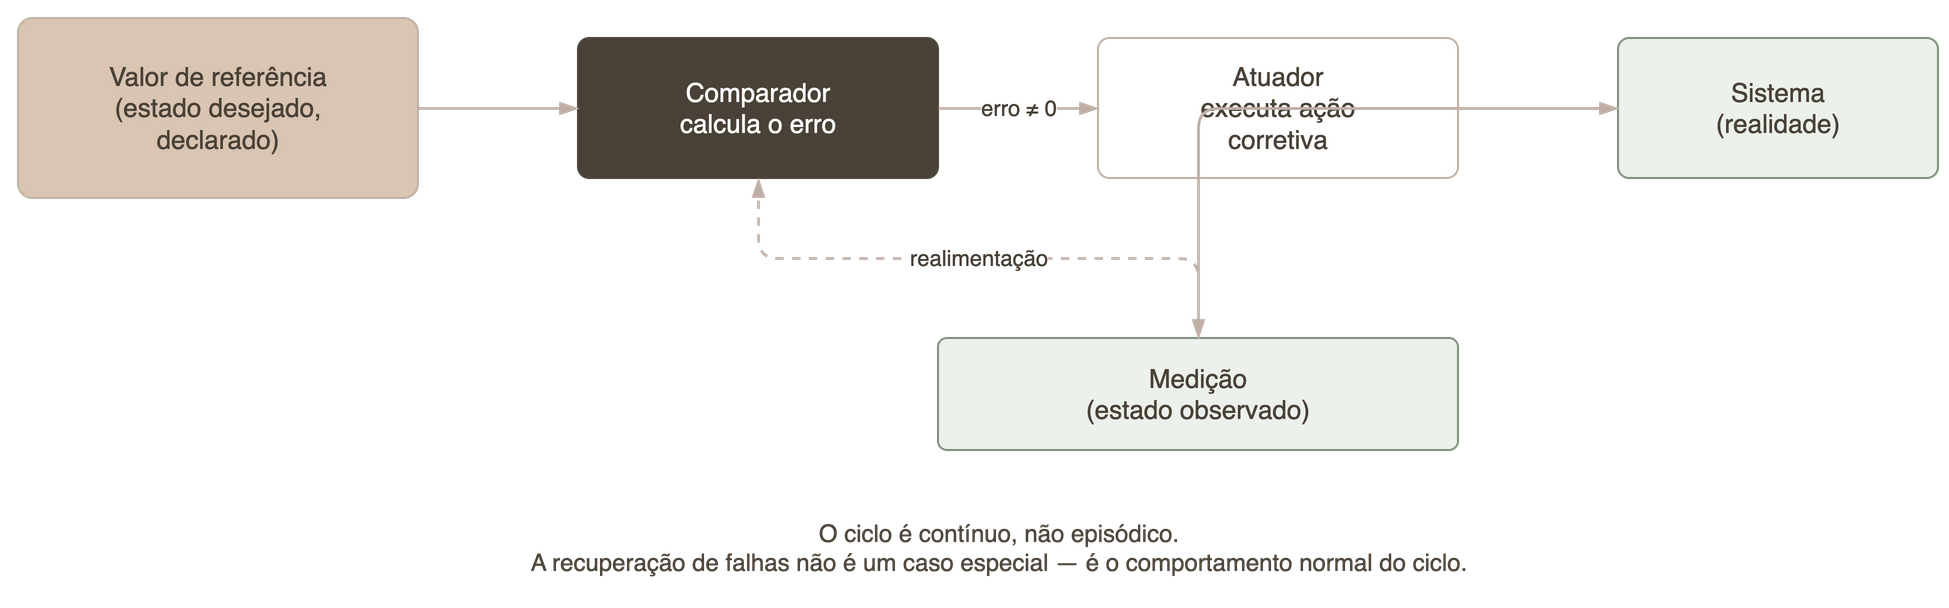
\includegraphics[width=0.97\textwidth,height=0.70\textheight,keepaspectratio]{../Diagramas/a01-ciclo-controlo.png}
\end{center}
\vfill
\end{frame}

\begin{frame}
\frametitle{Acoplamento entre componentes}
\begin{itemize}
    \setlength\itemsep{0.35cm}
    \item \textbf{Acoplamento}: medida da dependência entre componentes -- quanto é que a alteração ou falha de um afeta os outros.
    \item Distinguem-se várias dimensões: temporal (têm de estar ativos em simultâneo?), de localização, de formato de dados e de implementação.
    \item Reduzir acoplamento aumenta a capacidade de evoluir e de falhar isoladamente; aumenta também o número de componentes a gerir.
    \item Não existe um nível de acoplamento universalmente correto -- existe um nível adequado a um dado conjunto de requisitos.
\end{itemize}
\end{frame}

% ============================================================
\seccao{Parte 3}{O argumento económico}

\begin{frame}
\frametitle{Porque se consolida}
\begin{itemize}
    \setlength\itemsep{0.35cm}
    \item Um sistema dimensionado para o seu pico de procura permanece subutilizado durante a maior parte do tempo.
    \item Dimensionar para a média torna-o incapaz de responder ao pico.
    \item O dilema é insolúvel \emph{para um sistema isolado}. Deixa de o ser quando se agregam vários sistemas independentes.
    \item A consolidação não é apenas uma conveniência operacional: assenta numa propriedade estatística da agregação de procuras independentes.
\end{itemize}
\end{frame}



\begin{frame}
\frametitle{Quando a consolidação não compensa}
\begin{itemize}
    \setlength\itemsep{0.35cm}
    \item Agregar muitas procuras independentes torna a procura total proporcionalmente \emph{mais previsível} do que cada uma isoladamente.
    \item Daí resulta que a margem de segurança necessária, em proporção, diminui à medida que se agregam cargas -- é esta a base da economia de escala.
    \item A hipótese crítica é a \textbf{independência}. Se as cargas forem correlacionadas, por exemplo com pico à mesma hora, a previsibilidade desaparece e o ganho com ela.
    \item Um modelo é útil sobretudo por ser explícito quanto às condições em que deixa de se aplicar.
\end{itemize}
\end{frame}

\begin{frame}
\frametitle{Utilização e latência}
\begin{itemize}
    \setlength\itemsep{0.3cm}
    \item Uma intuição comum sugere que se deve operar a infraestrutura com utilização próxima de 100\%, para não desperdiçar.
    \item A teoria de filas de espera mostra que essa intuição está errada.
    \item Para um sistema elementar com chegadas e serviço exponenciais (modelo M/M/1), o tempo médio de resposta $R$ relaciona-se com o tempo de serviço $S$ e a utilização $\rho$ por
    \[
      R \;=\; \frac{S}{1-\rho}
    \]
    \item À medida que $\rho \rightarrow 1$, o tempo de resposta cresce sem limite.
\end{itemize}
\end{frame}

\begin{frame}
\frametitle{O que isto significa na prática}
\begin{itemize}
    \setlength\itemsep{0.3cm}
    \item Avaliando $R/S$ para valores crescentes de utilização:
    \begin{itemize}
      \item $\rho = 0{,}50 \;\Rightarrow\; R = 2S$
      \item $\rho = 0{,}80 \;\Rightarrow\; R = 5S$
      \item $\rho = 0{,}90 \;\Rightarrow\; R = 10S$
      \item $\rho = 0{,}99 \;\Rightarrow\; R = 100S$
    \end{itemize}
    \item A degradação não é linear.
    \item Operar com folga não é desperdício -- é o preço da previsibilidade da latência.
\end{itemize}
\end{frame}



\begin{frame}
\frametitle{O que torna a elasticidade útil}
\begin{itemize}
    \setlength\itemsep{0.35cm}
    \item \textbf{Elasticidade}: capacidade de ajustar a capacidade aprovisionada à procura observada, em ambos os sentidos.
    \item O seu valor depende de três grandezas: a amplitude da variação da procura, o tempo de reação do mecanismo de ajuste e a granularidade da unidade faturada.
    \item Se o tempo de reação for superior à duração do pico, a elasticidade não produz benefício.
\end{itemize}
\end{frame}

% ============================================================
\seccao{Parte 4}{O que é, afinal, \emph{cloud}}

\begin{frame}
\frametitle{Porque precisamos de uma definição}
\begin{itemize}
    \setlength\itemsep{0.35cm}
    \item O termo \emph{cloud} é usado com sentidos muito diferentes consoante o contexto -- comercial, técnico ou contratual.
    \item Num contexto de engenharia, um termo sem fronteiras definidas impede raciocínio rigoroso e comparação entre alternativas.
    \item A definição do NIST (Mell e Grance, 2011) é a referência habitual porque é \emph{operacional}: enuncia critérios verificáveis.
    \item Vamos analisá-la como se analisa qualquer definição: identificando o que inclui, o que exclui e o que deixa em aberto.
\end{itemize}
\end{frame}

\begin{frame}
\frametitle{As cinco características do NIST}
\begin{itemize}
    \setlength\itemsep{0.3cm}
    \item \textbf{Self-service sob procura} -- o consumidor aprovisiona sem intervenção humana do fornecedor.
    \item \textbf{Acesso alargado à rede} -- disponível através de mecanismos padronizados.
    \item \textbf{Partilha de recursos} (\emph{resource pooling}) -- recursos servem múltiplos consumidores, com atribuição dinâmica.
    \item \textbf{Elasticidade rápida} -- capacidade ajustável, em ambos os sentidos, com rapidez.
    \item \textbf{Serviço medido} -- o consumo é monitorizado e reportado de forma transparente.
\end{itemize}
\end{frame}

\begin{frame}
\frametitle{O que a definição realmente diz}
\begin{itemize}
    \setlength\itemsep{0.35cm}
    \item As cinco não são independentes: o \emph{serviço medido} é pré-condição do \emph{self-service} com responsabilização, e a \emph{partilha de recursos} é pré-condição da \emph{elasticidade}.
    \item Duas são de natureza técnica (partilha, elasticidade); três são de natureza \emph{organizacional} -- descrevem a relação entre fornecedor e consumidor.
    \item Consequência frequentemente ignorada: uma infraestrutura pode ser tecnicamente sofisticada e ainda assim não constituir uma \emph{cloud}, se o aprovisionamento exigir intervenção humana.
    \item A definição é, no essencial, sobre \textbf{modo de operação}, não sobre tecnologia empregue.
\end{itemize}
\end{frame}

\begin{frame}
\frametitle{O que significam IaaS, PaaS e SaaS}
\begin{itemize}
    \setlength\itemsep{0.4cm}
    \item \textbf{IaaS} --- \emph{Infrastructure as a Service}\newline
    {\small O fornecedor entrega recursos brutos: capacidade de computação, armazenamento e rede. O cliente instala e gere o sistema operativo e tudo o que corre acima dele.}
    \item \textbf{PaaS} --- \emph{Platform as a Service}\newline
    {\small O fornecedor entrega um ambiente de execução já pronto. O cliente entrega a aplicação e os dados, sem gerir o sistema operativo.}
    \item \textbf{SaaS} --- \emph{Software as a Service}\newline
    {\small O fornecedor entrega a aplicação a funcionar. Ao cliente resta configurar acessos e gerir os seus dados.}
\end{itemize}
\end{frame}

\begin{frame}
\frametitle{IaaS, PaaS e SaaS}
\begin{itemize}
    \setlength\itemsep{0.35cm}
    \item \textbf{IaaS}, \textbf{PaaS} e \textbf{SaaS} são habitualmente apresentados como níveis de abstração crescente.
    \item É mais produtivo lê-los como diferentes \textbf{repartições de responsabilidade} sobre uma mesma pilha de camadas.
    \item Em cada modelo desloca-se a fronteira entre o que o fornecedor gere e o que o consumidor gere.
    \item Cada deslocação troca \emph{controlo} por \emph{redução de encargo operacional} -- e é essa troca, não o nível de abstração em si, que fundamenta a escolha.
\end{itemize}
\end{frame}



\begin{frame}
\frametitle{Onde fica a fronteira}
\vfill
\begin{center}
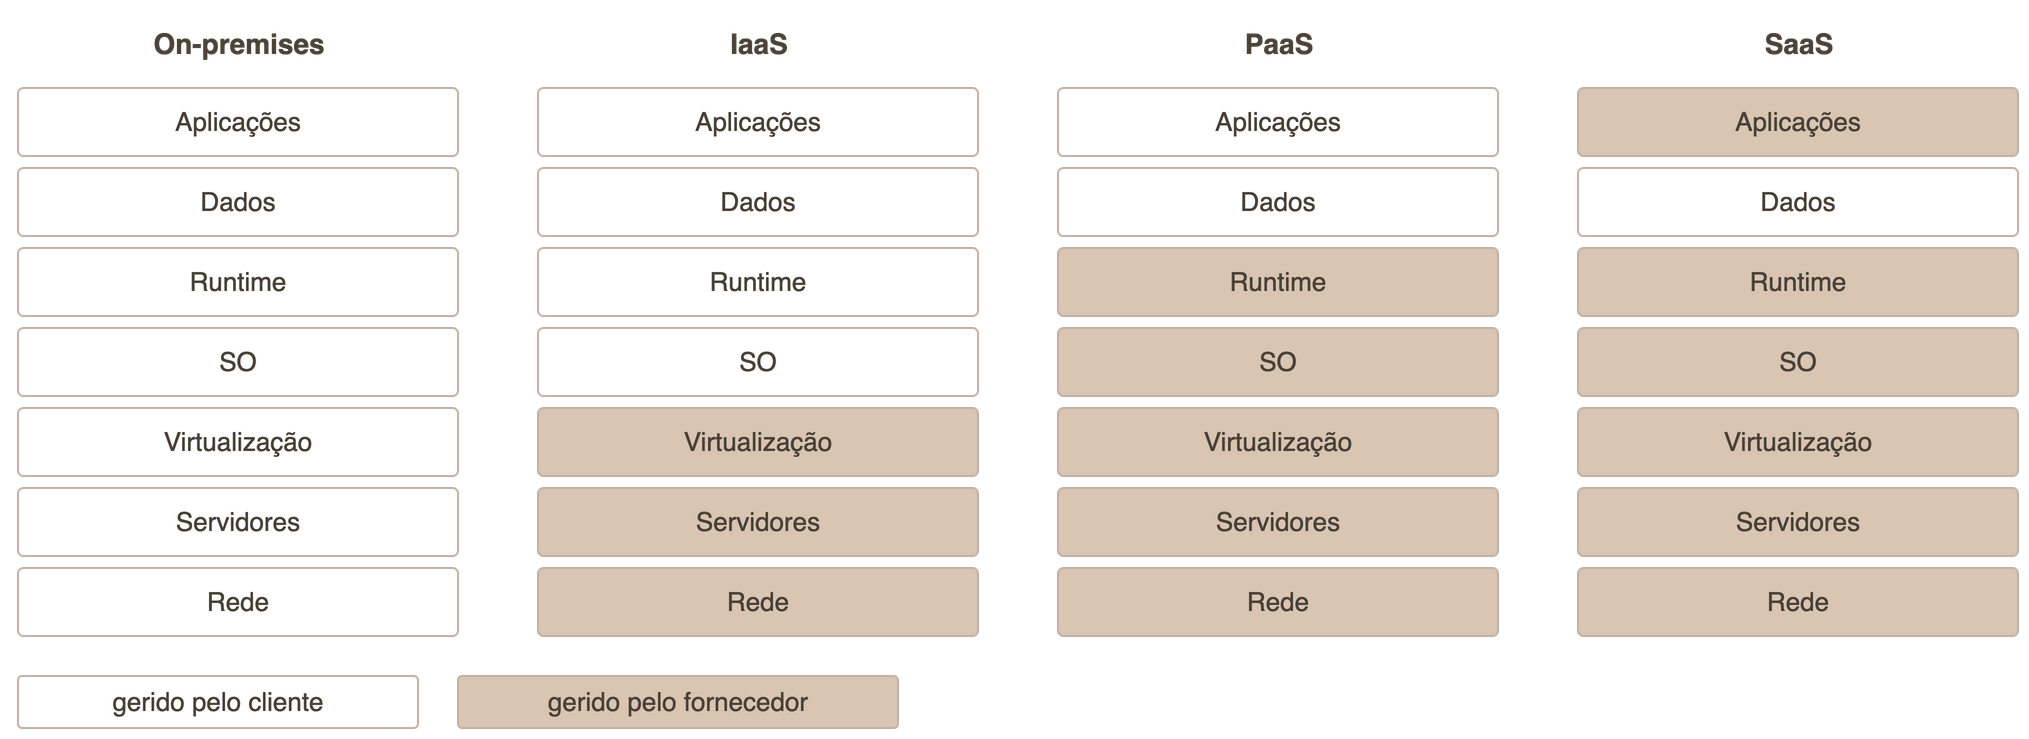
\includegraphics[width=0.97\textwidth,height=0.70\textheight,keepaspectratio]{../Diagramas/a01-modelos-servico.png}
\end{center}
\vfill
\end{frame}

\begin{frame}
\frametitle{O que a fronteira determina}
\begin{itemize}
    \setlength\itemsep{0.35cm}
    \item A fronteira determina simultaneamente a responsabilidade \emph{operacional} e a responsabilidade \emph{de segurança}.
    \item Uma fonte recorrente de incidentes é a suposição de que o que está acima da fronteira é assegurado por quem está abaixo dela.
    \item A fronteira determina também o \textbf{grau de dependência do fornecedor}: quanto mais alto o modelo, mais específicas as interfaces utilizadas, e mais dispendiosa a migração.
    \item Esta unidade curricular situa-se predominantemente ao nível de \textbf{IaaS} -- a camada onde a infraestrutura é explicitamente construída e administrada.
\end{itemize}
\end{frame}

\begin{frame}
\frametitle{Pública, privada, híbrida}
\begin{itemize}
    \setlength\itemsep{0.35cm}
    \item \textbf{Pública}, \textbf{privada}, \textbf{híbrida} e \textbf{comunitária} distinguem-se pelo \emph{locus de controlo} e pelo conjunto de consumidores servidos.
    \item A distinção não é primariamente técnica: as mesmas tecnologias podem sustentar qualquer um dos modelos.
    \item Os critérios de escolha são tipicamente de natureza regulatória, contratual ou de governação -- por exemplo, requisitos de localização dos dados.
    \item O modelo híbrido introduz uma dificuldade específica: a necessidade de manter coerência operacional entre ambientes com modelos de gestão distintos.
\end{itemize}
\end{frame}

\begin{frame}
\frametitle{O que a definição deixa de fora}
\begin{itemize}
    \setlength\itemsep{0.35cm}
    \item Nada diz sobre \textbf{desempenho}: um sistema lento pode satisfazer integralmente as cinco características.
    \item Nada diz sobre \textbf{dependabilidade}: a definição é ortogonal à fiabilidade do serviço.
    \item Nada diz sobre \textbf{custo}: a elasticidade não implica economia.
    \item Estas dimensões, ausentes da definição, são precisamente aquelas em que reside o trabalho de engenharia -- e o objeto das partes seguintes desta aula.
\end{itemize}
\end{frame}

% ============================================================
\seccao{Parte 5}{Qualidade e dependabilidade}

\begin{frame}
\frametitle{Quando um atributo se torna requisito}
\begin{itemize}
    \setlength\itemsep{0.35cm}
    \item Requisitos \emph{funcionais} dizem o que o sistema faz; \emph{atributos de qualidade} dizem com que propriedades o faz.
    \item Em infraestrutura, são os atributos de qualidade que determinam a arquitetura -- a funcionalidade é frequentemente trivial.
    \item Um atributo só é um requisito quando é \textbf{quantificado e verificável}. «O sistema deve ser fiável» não é um requisito: não é possível verificar se foi cumprido.
    \item Tornar um atributo operacional exige definir a grandeza medida, o método de medição e o valor de referência.
\end{itemize}
\end{frame}

\begin{frame}
\frametitle{Os atributos de dependabilidade}
\begin{itemize}
    \setlength\itemsep{0.3cm}
    \item Quadro de referência estabelecido por Avižienis, Laprie, Randell e Landwehr (2004).
    \item \textbf{Dependabilidade}: capacidade de um sistema merecer confiança justificada no serviço que presta.
    \item Decompõe-se em atributos mensuráveis:
    \begin{itemize}
      \item \emph{Disponibilidade} -- prontidão para prestar serviço correto.
      \item \emph{Fiabilidade} -- continuidade do serviço correto ao longo do tempo.
      \item \emph{Integridade} -- ausência de alterações impróprias do estado.
      \item \emph{Manutenibilidade} -- aptidão para ser reparado e modificado.
    \end{itemize}
\end{itemize}
\end{frame}

\begin{frame}
\frametitle{Disponibilidade não é fiabilidade}
\begin{itemize}
    \setlength\itemsep{0.35cm}
    \item \textbf{Disponibilidade} é uma proporção de tempo; \textbf{fiabilidade} é a probabilidade de funcionamento ininterrupto durante um intervalo.
    \item Um sistema que falha frequentemente mas recupera em segundos pode ter disponibilidade elevada e fiabilidade baixa.
    \item Um sistema que falha raramente mas demora dias a recuperar pode ter fiabilidade elevada e disponibilidade baixa.
    \item A distinção é determinante: os dois atributos exigem investimentos diferentes -- respetivamente, em recuperação rápida e em prevenção de falhas.
\end{itemize}
\end{frame}

\begin{frame}
\frametitle{Falta, erro e falha}
\begin{itemize}
    \setlength\itemsep{0.35cm}
    \item \textbf{Falta} (\emph{fault}) -- a causa adjudicada ou hipotética de um erro. Pode permanecer latente indefinidamente.
    \item \textbf{Erro} (\emph{error}) -- desvio do estado do sistema relativamente ao estado correto. É a manifestação interna da falta.
    \item \textbf{Falha} (\emph{failure}) -- o serviço prestado desvia-se do serviço correto. É a manifestação externa do erro.
    \item A cadeia \emph{não} é determinística: uma falta pode nunca produzir erro, e um erro pode nunca propagar-se até à falha.
    \item Os mecanismos de tolerância a falhas atuam precisamente interrompendo esta cadeia.
\end{itemize}
\end{frame}

\begin{frame}
\frametitle{Como uma falta chega a falha}
\vfill
\begin{center}
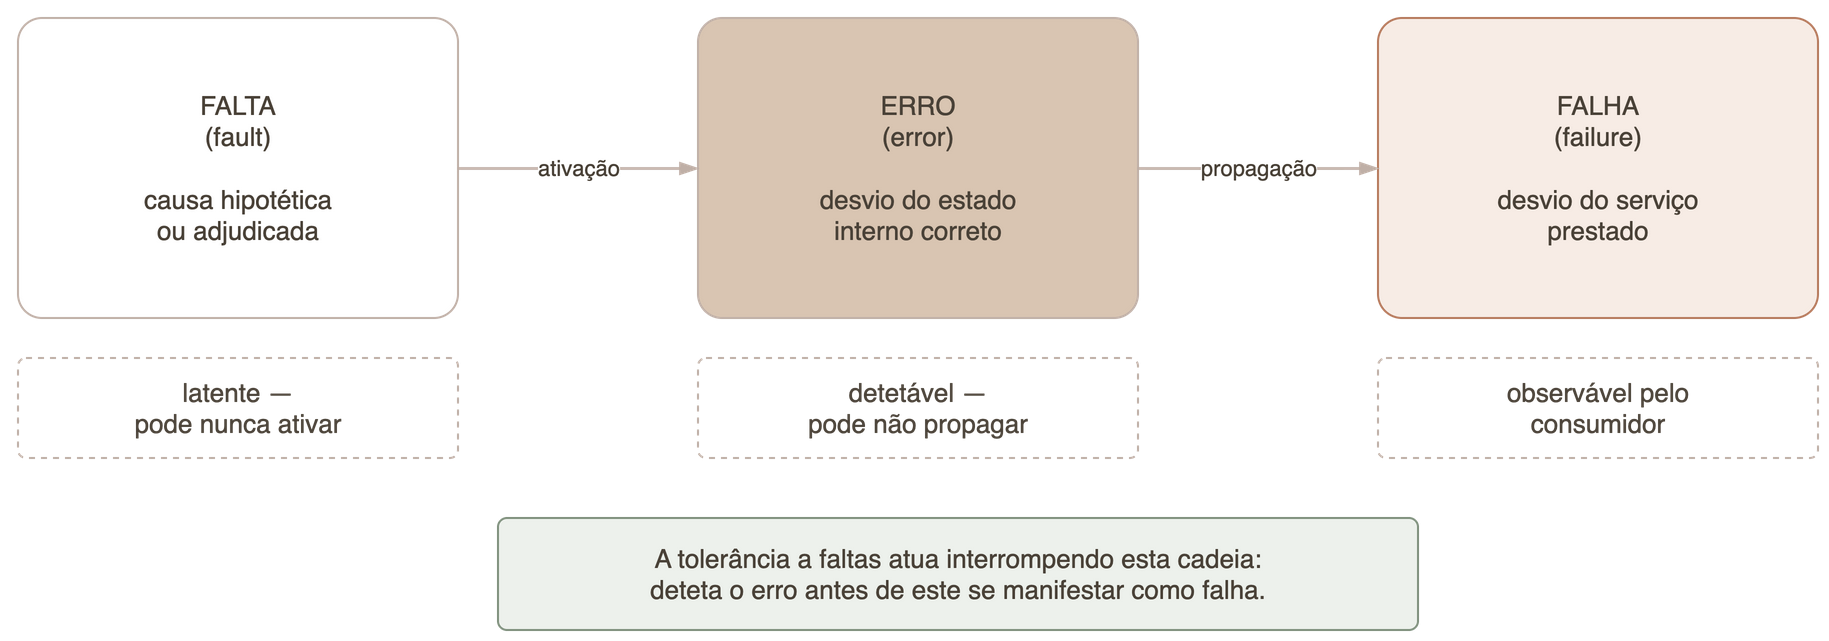
\includegraphics[width=0.97\textwidth,height=0.70\textheight,keepaspectratio]{../Diagramas/a01-falta-erro-falha.png}
\end{center}
\vfill
\end{frame}

\begin{frame}
\frametitle{Modelos de falta}
\begin{itemize}
    \setlength\itemsep{0.3cm}
    \item Um sistema tolerante a falhas é-o \emph{sempre relativamente a um modelo de falta declarado}. Não existe tolerância genérica.
    \item Modelos habituais, por ordem crescente de severidade:
    \begin{itemize}
      \item \textbf{Paragem} (\emph{crash}) -- o componente deixa de responder e não volta a agir.
      \item \textbf{Omissão} -- o componente ocasionalmente não responde.
      \item \textbf{Temporal} -- responde, mas fora do intervalo esperado.
      \item \textbf{Arbitrária} (bizantina) -- pode exibir qualquer comportamento, incluindo respostas incorretas e inconsistentes.
    \end{itemize}
    \item Quanto mais severo o modelo tolerado, mais dispendioso o mecanismo exigido.
\end{itemize}
\end{frame}

\begin{frame}
\frametitle{Quatro formas de lidar com faltas}
\begin{itemize}
    \setlength\itemsep{0.35cm}
    \item \textbf{Prevenção de faltas} -- impedir a sua introdução (processos de desenho, revisão, normas).
    \item \textbf{Tolerância a faltas} -- assegurar serviço correto na presença de faltas (redundância, deteção e recuperação).
    \item \textbf{Remoção de faltas} -- reduzir número e severidade (verificação, teste, diagnóstico).
    \item \textbf{Previsão de faltas} -- estimar incidência e consequências (modelos, análise estatística).
    \item Uma arquitetura séria emprega os quatro. Concentrar o esforço apenas na tolerância é um erro comum e dispendioso.
\end{itemize}
\end{frame}

\begin{frame}
\frametitle{Quando a redundância não chega}
\begin{itemize}
    \setlength\itemsep{0.35cm}
    \item A tolerância a faltas assenta em redundância -- de componentes, de informação ou de tempo.
    \item A sua eficácia depende de uma hipótese frequentemente implícita: a \textbf{independência das faltas}.
    \item Réplicas que partilham alimentação, rede, versão de software ou defeito de desenho falham em conjunto. A redundância aparente não se traduz em tolerância real.
    \item \textbf{Falta de modo comum}: aquela que afeta simultaneamente todas as réplicas. É o limite fundamental de qualquer esquema de redundância.
\end{itemize}
\end{frame}

\begin{frame}
\frametitle{SLI, SLO e SLA}
\begin{itemize}
    \setlength\itemsep{0.35cm}
    \item \textbf{SLI} (\emph{Service Level Indicator}) -- uma grandeza efetivamente medida, com definição operacional precisa.
    \item \textbf{SLO} (\emph{Service Level Objective}) -- um valor de referência para esse indicador, assumido internamente.
    \item \textbf{SLA} (\emph{Service Level Agreement}) -- um compromisso contratual, com consequências definidas em caso de incumprimento.
    \item A ordem importa: sem indicador não há objetivo verificável, e sem objetivo o acordo é inexequível.
    \item Confundir os três é uma das origens mais comuns de conflito entre equipas técnicas e a organização.
\end{itemize}
\end{frame}

\begin{frame}
\frametitle{Error budget}
\begin{itemize}
    \setlength\itemsep{0.35cm}
    \item Um SLO inferior a 100\% define, por complemento, uma quantidade admissível de indisponibilidade: o \textbf{orçamento de erro}.
    \item Um objetivo de 99,9\% num trimestre corresponde a um orçamento de aproximadamente 2,2 horas nesse período.
    \item A sua função é converter uma discussão qualitativa -- «devemos arriscar esta alteração?» -- numa decisão com critério explícito.
    \item Enquanto houver orçamento, a mudança é admissível; esgotado o orçamento, a prioridade desloca-se para a estabilização.
    \item Torna visível que fiabilidade e velocidade de mudança são grandezas em tensão, e não objetivos independentes.
\end{itemize}
\end{frame}

\begin{frame}
\frametitle{Atributos que competem entre si}
\begin{itemize}
    \setlength\itemsep{0.3cm}
    \item Atributos de qualidade raramente são independentes; melhorar um degrada tipicamente outro.
    \begin{itemize}
      \item Consistência forte entre réplicas custa latência.
      \item Isolamento forte entre consumidores custa eficiência de utilização.
      \item Redundância custa recursos e complexidade operacional.
      \item Segurança custa, quase sempre, conveniência.
    \end{itemize}
    \item Não há arquitetura ótima em abstrato -- há arquiteturas adequadas a uma ponderação declarada de requisitos.
    \item \textbf{Explicitar a ponderação é parte do trabalho de engenharia}, não um preliminar dele.
\end{itemize}
\end{frame}

% ============================================================
\seccao{Parte 6}{O fio condutor do semestre}

\begin{frame}
\frametitle{Como os blocos se encadeiam}
\begin{itemize}
    \setlength\itemsep{0.3cm}
    \item \textbf{C1} estabelece o substrato: recursos finitos, restrições físicas, modelos de operação.
    \item \textbf{C2} introduz o mecanismo que permite parti-los: virtualização e containerização.
    \item \textbf{C3} trata da gestão em escala: orquestração, rede programável, automatização.
    \item \textbf{C4} passa dos recursos aos serviços: disponibilidade, escala, desacoplamento.
    \item \textbf{C5} trata do estado, que é o que resiste à abstração: armazenamento.
    \item \textbf{C6} fecha o ciclo: observar e administrar o que foi construído.
\end{itemize}
\end{frame}

\begin{frame}
\frametitle{Perguntas que vão reaparecer}
\begin{itemize}
    \setlength\itemsep{0.3cm}
    \item Que recurso está a ser partilhado, e por que mecanismo?
    \item Que abstração está a ser oferecida, e em que condições deixa de se sustentar?
    \item Que modelo de falta é tolerado, e a que custo?
    \item O estado desejado é declarado ou construído por uma sequência de ações?
    \item Que indicador permite verificar que o sistema está a fazer o que se pretende?
    \item Reconhecer estas questões em contextos novos é, mais do que memorizar tecnologias, o objetivo da UC.
\end{itemize}
\end{frame}













\end{document}
